\begin{circuitikz}[
        american, 
        >={Latex[length=5mm, width=2mm]},
        %>=latex,
        alt={}
    ]

        \begin{axis}[
            width=6in,
            height=4in,
            axis lines=middle,
            color=BakerBlack,           % Sets default draw/text color for the axis
            axis line style={BakerBlack},
            tick style={BakerBlack},
            label style={BakerBlack},
            tick label style={BakerBlack},
            xlabel={Time ($t$)},        
            xlabel style={at={(ticklabel* cs:1)}, anchor=west},
            ylabel={Voltage ($V$)},
            ylabel near ticks,
            xmin=0, xmax=370,
            ymin=-200, ymax=200,
            xtick={0, 90, 180, 270, 360},
            xticklabels={$0^\circ$, $90^\circ$, $180^\circ$, $270^\circ$, $360^\circ$},
            ytick={-169.706, 0, 169.706},
            yticklabels={},
            grid=none,
            %grid style={dashed, gray!30},
            enlargelimits=false,
            clip=false
        ]
            % pgfplots trig functions expect degrees by default
            \addplot[domain=0:180, samples=100, ultra thick, LakeBlue] {169.706 * sin(x)};

            \addplot[domain=180:360, samples=100, ultra thick, BakerADARed] {169.706 * sin(x)};

            \node[
                above
            ]
            (A) 
            at (0,200)
            {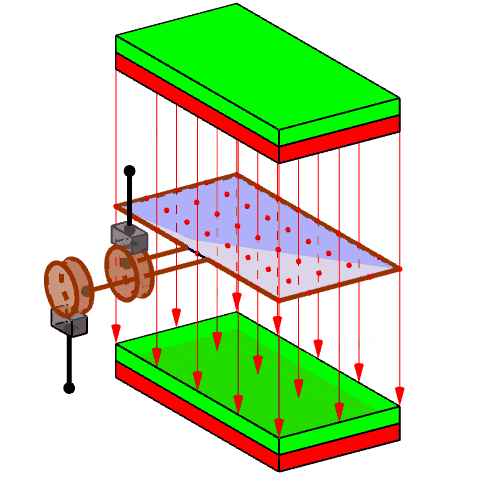
\includegraphics[width=3cm]{./Electric-generator-animation-5.png}};

            \node[
                above
            ]
            (B) 
            at (90,200)
            {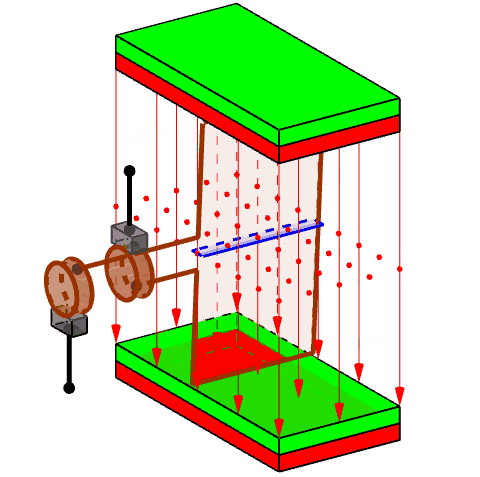
\includegraphics[width=3cm]{./Electric-generator-animation-17.png}};

            \node[
                above
            ]
            (C) 
            at (180,200)
            {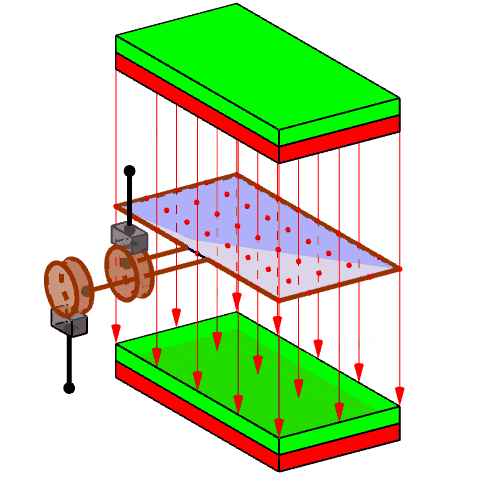
\includegraphics[width=3cm]{./Electric-generator-animation-5.png}};

            \node[
                above
            ]
            (D) 
            at (270,200)
            {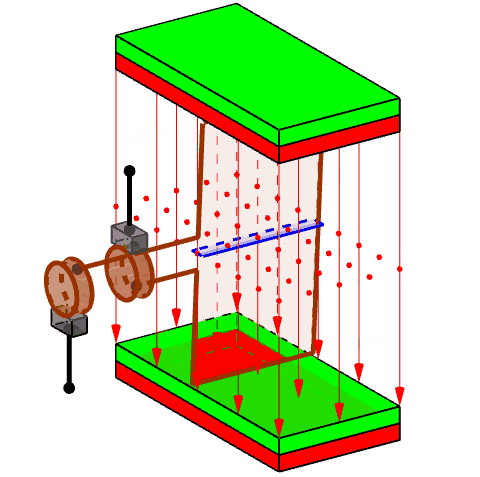
\includegraphics[width=3cm]{./Electric-generator-animation-17.png}};

            \node[
                above
            ]
            (E) 
            at (360,200)
            {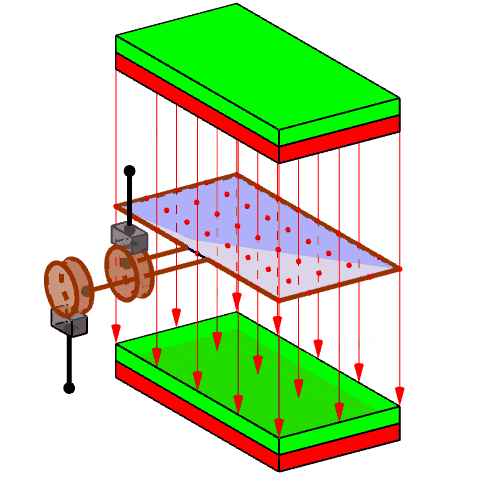
\includegraphics[width=3cm]{./Electric-generator-animation-5.png}};

            \draw[
                BakerADARed,
                dashed
            ]
            (B.south)
            -- (90,0)
            node[
                pos=0.75,
                right,
                text=BakerBlack
            ]
            {1/4 turn};

            \draw[
                BakerADARed,
                dashed
            ]
            (C.south)
            -- (180,0)
            node[
                pos=0.75,
                right,
                text=BakerBlack
            ]
            {1/2 turn};

            \draw[
                BakerADARed,
                dashed
            ]
            (D.south)
            -- (270,0)
            node[
                pos=0.75,
                right,
                text=BakerBlack
            ]
            {3/4 turn};

            \draw[
                BakerADARed,
                dashed
            ]
            (E.south)
            -- (360,0)
            node[
                pos=0.75,
                right,
                text=BakerBlack
            ]
            {1 turn};
            
            \draw[
                UpNorthGreen,
                dashed
            ]
            (180,0)
            -- (180,-60)
            coordinate[pos=0.75](alt);

            \draw[
                UpNorthGreen,
                <->
            ]
            (alt)
            -- (alt -| A.south)
            node[
                text=BakerBlack,
                pos=0.5,
                below
            ]{1 alternation};

            \draw[
                UpNorthGreen,
                dashed
            ]
            (360,0)
            -- (360,-230)
            coordinate[pos=0.875](cycle);

            \draw[
                UpNorthGreen,
                <->
            ]
            (cycle)
            -- (cycle -| A.south)
            node[
                text=BakerBlack,
                pos=0.5,
                below
            ]{1 cycle};
        
        \end{axis}

\end{circuitikz}